\subsection{Fragen und Antworten zum Text von \textcite{luke_getting_2005}}
\subsubsection{Auf welche Diskrepanz innerhalb der community-psychologischen Forschung und Anwendung weist Luke hin? Welche Gr"unde werden f"ur diese Diskrepanz aufgef"uhrt?}
In der Theorie wird die Ber"ucksichtigung des Kontextes gefordert, es werden allerdings kaum kontextuellen Methoden angewandt. Mogliche Gr"unde:
\begin{itemize}
  \item Lehrende der (Community) Psychologie lehren diese Methoden nicht
  \item es sind typischerweise andere Disziplinen, in denen kontextuelle Methoden benutzt werden
  \item \emph{Rule of the Hammer}: wenn das einzige Werkzeug ein hammer ist, dann benutz ich den f"ur alles
\end{itemize}

\subsubsection{Skizzieren Sie das von Luke (2005) gew"ahlte Verfahren, um zu untersuchen, ob sich der Methodeneinsatz "uber einen Zeitraum von zwanzig Jahren im Bereich der Community Psychology ver"andert hat. Was sind die zentralen Befunde dieser Analyse?}
Untersucht wurde die Verwendung statistischer Methoden in Studien, die im American Journal of Community Psychology (AJCP) ver"offentlicht wurden, und das "uber einen Zeitraum von $6$ Jahren, aufgeteteilt auf $2$ Zeitr"aume (um eine Ver"anderung "uber die  Zeit entdecken zu k"onnen).

Auch wenn sich die Methoden etwas ver"andert haben: es werden immer noch weit mehr traditionelle Verfahren (ANOVA, Korrelationen) verwendet. (Siehe Fig. \ref{fig:luke1})

\begin{figure}[hb!]
        \begin{center}
                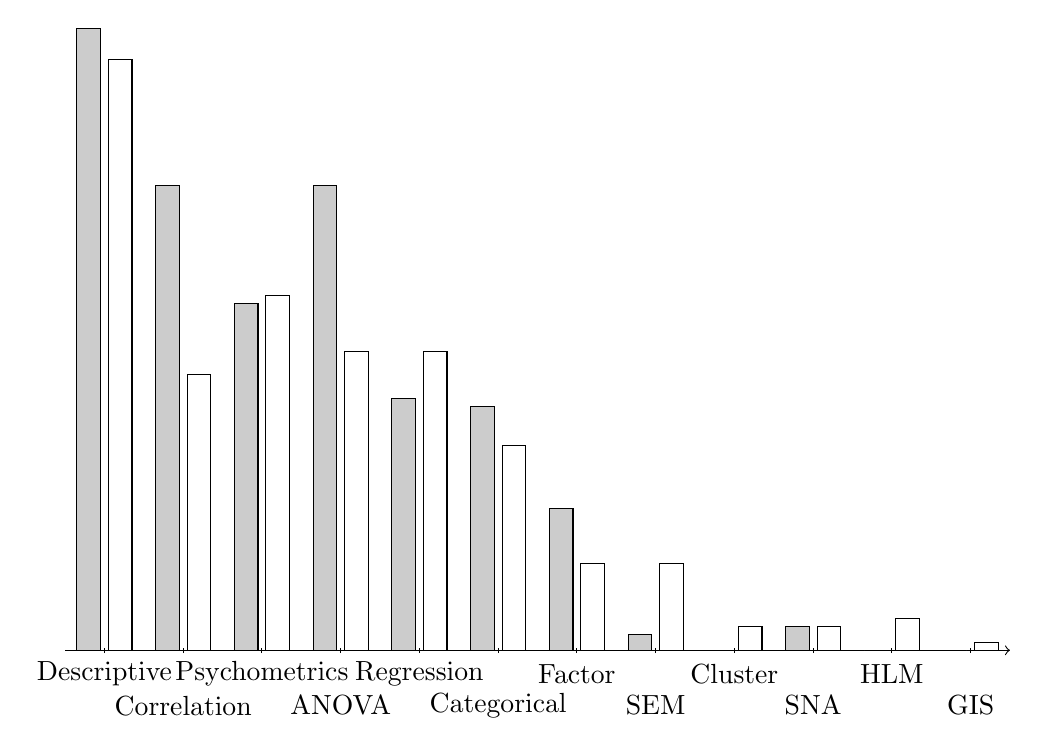
\begin{tikzpicture}[text/.style={font=\tiny},
                        t1/.style={fill=black!20},
                        ]
                        %x-Achse und Ticks
                        \draw [->] (-6,0) -- (+6,0);
                        \foreach \x in {-5.5, -4.5, -3.5, -2.5, -1.5, -0.5, 0.5, 1.5, 2.5, 3.5, 4.5, 5.5} 
                        \draw [-] (\x,-1pt) -- (\x,+1pt);
                        %Beschriftung
                        \node at (-5.5, -0.3) {Descriptive};
                        \node at (-4.5, -0.7) {Correlation};
                        \node at (-3.5, -0.3){Psychometrics};
                        \node at (-2.5, -0.7) {ANOVA};
                        \node at (-1.5, -0.3) {Regression};
                        \node at (-0.5, -0.7) {Categorical};
                        \node at (+0.5, -0.3) {Factor};
                        \node at (+1.5, -0.7) {SEM};
                        \node at (+2.5, -0.3) {Cluster};
                        \node at (+3.5, -0.7) {SNA};
                        \node at (+4.5, -0.3) {HLM};
                        \node at (+5.5, -0.7) {GIS};
                        %Balken fuer ersten Zeitraum
                        \draw [t1] (-5.85,0) rectangle (-5.55,7.9);
                        \draw [t1] (-4.85,0) rectangle (-4.55,5.9);
                        \draw [t1] (-3.85,0) rectangle (-3.55,4.4);
                        \draw [t1] (-2.85,0) rectangle (-2.55,5.9);
                        \draw [t1] (-1.85,0) rectangle (-1.55,3.2);
                        \draw [t1] (-0.85,0) rectangle (-0.55,3.1);
                        \draw [t1] (+0.15,0) rectangle (+0.45,1.8);
                        \draw [t1] (+1.15,0) rectangle (+1.45,0.2);
                        \draw [t1] (+2.15,0) rectangle (+2.45,0.0);
                        \draw [t1] (+3.15,0) rectangle (+3.45,0.3);
                        \draw [t1] (+4.15,0) rectangle (+4.45,0.0);
                        \draw [t1] (+5.15,0) rectangle (+5.45,0.0);
                        %Balken fuer den zweiten Zeitraum
                        \draw (-5.45,0) rectangle (-5.15,7.5);
                        \draw (-4.45,0) rectangle (-4.15,3.5);
                        \draw (-3.45,0) rectangle (-3.15,4.5);
                        \draw (-2.45,0) rectangle (-2.15,3.8);
                        \draw (-1.45,0) rectangle (-1.15,3.8);
                        \draw (-0.45,0) rectangle (-0.15,2.6);
                        \draw (+0.55,0) rectangle (+0.85,1.1);
                        \draw (+1.55,0) rectangle (+1.85,1.1);
                        \draw (+2.55,0) rectangle (+2.85,0.3);
                        \draw (+3.55,0) rectangle (+3.85,0.3);
                        \draw (+4.55,0) rectangle (+4.85,0.4);
                        \draw (+5.55,0) rectangle (+5.85,0.1);
                        %\pgfpathrectangle{-5.9,0}{-5.4,0.79}
                \end{tikzpicture}
        \end{center}
        \caption{Ergebnisse der Analyse von \textcite{luke_getting_2005}. Die dunklen Balken repr"asentieren den ersten Zeitraum, die hellen den zweiten.}
        \label{fig:luke1}
\end{figure}

\subsubsection{Welche Probleme ergeben sich durch die Vernachl"assigung des Kontexts im Rahmen des Allgemeinen Linearen Modells?}
\begin{itemize}
  \item korrelierte Fehler durch abh"angige Messungen
  \item gleiche Regressionskoeffizienten f"ur unterschiedliche Kontexte
\end{itemize}

\subsubsection{Skizzieren Sie das Prinzip der Mehrebenenanalyse. Welche Vor- und Nachteile hat dieses Analyseverfahren? F"ur welche community-psychologischen Fragestellungen kann dieses Verfahren verwendet werden?}
Die Mehrebenenanalyse ist ein allgemeines regressionsbasiertes Verfahren zur Abbildung hierarchischer Daten. Es ist leider, leider etwas komplizierter als eine Regressionsanalyse (Nachteil), erlaubt aber zwei Dinge:

\begin{itemize}
  \item Level-$1$-Koeffizienten werden auf Level-$2$ zu AVs. Das erlaubt unterschiedliche Effekt in unterschiedlichen Kontexten.
  \item Es wird genau angezeigt, welche Pr"adiktorvariablen auf welcher Ebene Varianz aufkl"aren.
\end{itemize}

\subsubsection{Wof"ur k“onnen Methoden des Geographic Information Systems (GIS) eingesetzt werden? Nennen Sie community-psychologischen Fragestellungen, die durch den Einsatz von GIS adressiert werden k"onnen!}
GIS ist eine quantitative Methode zur Erforschung des Kontextes.  GIS besteht aus einer Reihe von Datenbanken, Karten und statistischen Werkzeugen zur visuellen und quantitativen Bewertung von geographischen Informationen. Meist ist die Erstellung von Karten das Ziel, es k"onnen aber auch Kontextvariablen ausgearbeitet werden oder statistische Analysen r"aumlicher Beziehungen durchgef"uhrt werden. u den Einsatzm"oglichkeiten geh"oren:
\begin{itemize}
  \item Gemeindeentwicklung
  \item Abbildung von Verm"ogen der Gemeinde
  \item Bewertung der Community Gesundheit
  \item "Okologische Entwicklung
  \item Straftaten aufdecken
  \item Risikobehaftetes Gesundheitsverhalten aufdecken
\end{itemize}

\subsubsection{Welche Daten werden im Rahmen von Netzwerkanalysen (Social Network Analysis, SNA) ausgewertet?}
Basis bildet die Analyse von \emph{relationalen Daten}, also Informationen "uber Beziehungen zwischen einer Reihe von Akteuren. Hier liegt ein Unterschied zum Rest der Community Science, in der typischerweise Attribute von Daten gesammelt und analysiert werden – nicht deren Beziehungen.

\subsubsection{Was sind \emph{ego-centric networks}? Welche Vor- und Nachteile haben diese Netzwerke?}
Ego-centric networks sind allein durch die Perspektive eines einzelnen Mitglieds bestimmt. Die Dichte entspricht dem Anteil der Verbindungen in einem Netzwerk bezogen auf die gesamte m"ogliche Anzahl von Verbindungen.
Nachteile:\\
\begin{itemize}
  \item keine repr"asentative Abbildung vollst"andiger Netzwerke
  \item nur indirekte Beziehungen k"onnen untersucht werden
\end{itemize}

\subsubsection{Was wird mit \emph{Freeman’s betweenness index} (Wasserman \& Faust, 1994) ausgedr“uckt? Wie ist dieser Index definiert? Wie wird dieser Index interpretiert?}
Freemans betweenness index entspricht der \emph{betweenness centrality} (Intermediationszentralit“at). Er miss, wie oft ein einzelner Akteur in die Kommunikation zwischen zwei anderen Akteuren involviert ist. Der Wertebereich liegt zwischen $0$ und $1$. $1$ bedeutet, dass der Akteur Kontakt zu allen Akteuren eines Netzwerks hat. 

\subsubsection{Was wird mit dem \emph{network centralization index} ausgedr"uckt? Wie wird dieser Index definiert? Wie wird dieser Index interpretiert?}
Der network centralization index entspricht der \emph{Aggregation aller betweenness-Werte} der einzelnen Akteure zu einem einzigen Wert und liegt ebenfalls zwischen $0$ und $1$.\\ 
Er betr“agt $1$ (100\%), wenn ein Akteur die maximale betweenness (=Kontakt zu allen) aufweist und alle anderen Akteure einen betweenness-Index von $0$ haben.\\
Er betr“agt $0$, wenn alle Akteure den gleichen betweenness-Index haben.
\begin{itemize}
  \item Hohe Werte = hierarchische Kommunikationsstruktur im Netzwerk
  \item Niedrige Werte = flache Kommunikationsstruktur
\end{itemize}

\subsubsection{Skizzieren Sie das Prinzip der \emph{Clusteranalyse}. Welche Vor- und Nachteile hat dieses Analyseverfahren? F"ur welche community-psychologischen Fragestellungen kann dieses Verfahren verwendet werden?}
Mit der Clusteranalyse k"onnen Diversit"at und Heterogenit"at innerhalb von Daten aufgezeigt werden. Es werden Objekte (h"aufig Personen) nach Gemeinsamkeiten und Unterschieden "uber eine beliebige Anzahl von Variablen hinweg gruppiert.\\
Die CA ist eine explorative Technik, um unbekannte Heterogenit"at aufzuzeigen. Die steht im Gegensatz zu den traditionellen Modellen, in denen versucht wird, Heterogenit"at mittels Kovariaten zu kontrollieren.

\subsubsection{Welche Probleme diskutiert Luke (2005), die mit dem statistischen ``Kontrollieren'' von Heterogenit"at (z.B. durch Kovariaten) einhergehen?}
Fast schon philosophisch betrachtet f"uhrt statistische Kontrolle von Variablen zu einer ``Dekontextualisierung'' der Daten. Konkrete Probleme sind:
\begin{enumerate}
  \item Kontrolle von Heterogenit"at impliziert, dass die individuellen Unterschiede nicht von wissenschaftlichem Interesse sind. Dabei kann gerade die Heterogenit“at den interessantesten Teil der Studie ausmachen.
  \item Kontrolle von Heterogenit“at f"uhrt manchmal zu einer Art ``methodischer Faulheit'': Bestimmte Kovariaten sind immer im Modell enthalten, weil sie bereits in fr"uheren Studien immer aufgenommen wurden.
\end{enumerate}

\subsubsection{Worauf bezieht sich der Begriff  \emph{methodological consilience}?}
\emph{Consilience} ``misst'' wieviel eine Theorie erkl"art und kann genutzt werden um herauszufinden, wann eine Theorie mehr erkl"art als eine andere. Es ist ein erkenntnistheoretisches Konstrukt, das verwendet wird um die Angemessenheit wissenschaftlicher Theorien zu beurteilen.\\
\emph{Methodological Consilience} ist eine Erweiterung dieser Idee: Die Untersuchung der Angemessenheit von wissenschaftlichen Methoden zur Analyse der Daten. Ein Modell ist dann erfolgreich, wenn es besonders viel Varianz aufkl"art.
